% !TeX spellcheck = de_DE
%% 
%% This is file 'beamer_sample.tex'
%% 	
%% by Mathias Winkel
%%
%% Problems, bugs and comments to 
%% mathias.winkel2@uni-rostock.de
%%
\RequirePackage{fix-cm} % because of font size substituion warnings
\documentclass[10pt]{beamer} % die 10pt sollten festgelegt bleiben, da dies die Groesse der Mathematikschrift etc. beeinflusst

\usepackage[ngerman]{babel}  % deutsche Bezeichnungen und Trennung etc
\usepackage[utf8]{inputenc}
\usepackage[T1]{fontenc}
\usepackage{csquotes}
\usepackage{hyperref}        % interne Hyperlinks
\usepackage[scaled]{beramono}
\usepackage{microtype}
\usepackage{listings}
\usepackage{ragged2e}
\usepackage{marvosym}
\usepackage{xcolor}
\usepackage{pgffor}

%******************************************
% For giving image sources, see http://tex.stackexchange.com/a/48485
\usepackage[absolute,overlay]{textpos}
\setbeamercolor{framesource}{fg=gray}
\setbeamerfont{framesource}{size=\tiny}

\setbeamercolor{plain}{fg=black,bg=white}

\newcommand{\source}[1]{\begin{textblock*}{4cm}(8.2cm,8.6cm)
		\begin{beamercolorbox}[ht=0.5cm,right]{framesource}
			\usebeamerfont{framesource}\usebeamercolor[fg]{framesource} Quelle: {#1}
		\end{beamercolorbox}
	\end{textblock*}}
%******************************************

\lstdefinestyle{customc}{
	tabsize=2,
	belowcaptionskip=1\baselineskip,
	breaklines=true,
	xleftmargin=\parindent,
	language=C,
	showstringspaces=false,
	basicstyle=\scriptsize\ttfamily,
	keywordstyle=\bfseries\color{green!40!black},
	commentstyle=\itshape\color{purple!40!black},
	identifierstyle=\color{blue},
	stringstyle=\color{orange},
}

\lstset{escapechar=@,style=customc}

\definecolor{links}{HTML}{2A1B81}
\hypersetup{colorlinks,linkcolor=,urlcolor=structure.fg}

\newcommand{\framefrompdf}[2]{
	\begin{frame}[plain]
		\hspace*{-8.5pt}
		\begin{beamercolorbox}[wd=\paperwidth,ht=\paperheight]{plain}
			\makebox[\paperwidth]{\hspace{8.5pt}\includegraphics[page=#2,width=\paperwidth]{#1}}
		\end{beamercolorbox}
	\end{frame}
}

\newcommand{\framesfrompdf}[3]{
	\foreach \n in {#2,...,#3}{\framefrompdf{#1}{\n}}
}

\newcommand{\framesfrompdfclipped}[8]{
	\foreach \n in {#2,...,#3}{
		\begin{frame}[plain]
			\vspace*{-18pt}\hspace*{-8.5pt}
			\makebox[\linewidth]{\includegraphics[page=\n,width=#8,clip,trim = #4 #5 #6 #7]{#1}}
		\end{frame}
	}
}

\newcommand{\picturefrompdf}[7]{
	\begin{center}
		%trim option's parameter order: left bottom right top
		\includegraphics[page=#2,width=#7,clip,trim = #3 #4 #5 #6]{#1} 
	\end{center}
}

\newcommand{\rto}{$\Rightarrow$ }

\newcommand{\emp}[1]{{\color{orange}{#1}}}

\newcommand{\img}[2]{
	\centering
	\includegraphics[#2]{figures/#1}
}

\newcommand{\questions}{
\begin{frame}
	
	\centering
	\Large
	Fragen?

\end{frame}
}

\newenvironment{task}[1]{
	\begin{block}{\textbf{Aufgabe} \hfill #1}
}{
	\end{block}
}

\AtBeginSection[]
{
	\begin{frame}{Plan für heute}
		\tableofcontents[currentsection]
	\end{frame}
}

\usepackage[uni,footuni,headlogo]{./unirostock/beamerthemeRostock}
% erster Parameter: Farbschema
%        moegliche Werte (nomen est omen): uni, inf, msf, ief, mnf, mef, juf, wsf, auf, thf, phf
%        Standardwert: uni
% zweiter Parameter: Fusszeile
%        moegliche Werte: footuni (Standard) - Fusszeile nach Handbuch des CD
%                         foottitle          - Autor und Title in der Fusszeile
%                         footheadings       - lebende Ueberschriften in der Fusszeile
%                         footuniheadings    - Autor und Uni sowie lebende Ueberschriften in der Fusszeile
% dritter Parameter: Kopfzeile
%        moegliche Werte: headlogo (Standard)- Inhalt von \mylogo in der Kopfzeile
%                         headtitle          - Vortragstitel
%                         headframetitle     - Folientitel
%                         headframesubtitle  - Folientitel und -untertitel
%        bitte nicht mehrere Varianten gleichzeitig angeben :-)

\setbeamercovered{invisible}
\addtobeamertemplate{block begin}{}{\justifying}

%%%%%%%%%%%% Festlegung der Titelseite %%%%%%%%%%%%%%%%%%%%%%%%%%%%%%%%%
\title[]{Imperative Programmierung}

\subtitle{Übung}

\author{\textsc{Tom Warnke}}

\institute{Universität Rostock, Institut für Informatik}

\titlegraphic{}

% ein alternatives Titelbild kann mittels 
%\titleimage{Dateiname.xyz}
% angegeben werden (auf vernuenftiges Seitenformat und Kontrastwerte achten, Skalierung und Abschneiden der oberen rechten Ecke passieren automatisch)
\titleimage{}

%%%%%%%%%%%% Festlegungen fuer Kopf- und Fusszeile %%%%%%%%%%%%%%%%%%%%
% Institutsname f\"ur die Fusszeile (nur wenn bei Paketeinbindung 'footuni' angegeben ist)
\footinstitute{Fakultät für Informatik und Elektrotechnik, Institut für Informatik}
% eigenes Logo oben rechts hinzufuegen (bitte auf vernuenftiges Format achten - ein zu hohes Logo verschiebt das Layout)
\renewcommand{\mylogo}{}

%%%%%%%%%%%%%%%%%%%%%%%%%%%%%%%%%%%%%%%%%%%%%%%%%%%%%%%%%%%%%%%%%%%%%%%

\date{}

%%%%%%%%%%%%%%%%%%%%%%%%%%%%%%%%%%%%%%%%%%%%%%%%%%%%%%%%%%%%%%%%%%%%%%%
\begin{document}

\maketitle

\begin{frame}{Plan für heute}

	\tableofcontents

\end{frame}

\section{Imperative Programmierung mit Stil}

\begin{frame}{Imperative Programmierung mit Stil}{K\&R über Einrückung, Klammern, \ldots}
	
	\enquote{The body of a while can be one or more statements enclosed in braces or a single statement without braces.	
		In either case, we will always indent the statements controlled by the while by one tab stop
		(which we have shown as four spaces) so you can see at a glance which statements are inside
		the loop. \emp{The indentation emphasizes the logical structure of the program.} Although C
		compilers do not care about how a program looks, \emp{proper indentation and spacing are critical
		in making programs easy for people to read}. We recommend writing only one statement per
		line, and using blanks around operators to clarify grouping. The position of braces is less
		important, although people hold passionate beliefs. We have chosen one of several popular
		styles. Pick a style that suits you, then use it consistently.}
	
\end{frame}

\begin{frame}[fragile]{Einfache Anweisungen}

	\begin{columns}
	\begin{column}{.4\textwidth}
	
	\begin{lstlisting}[gobble=4]
		if(a > b) max = a;
	\end{lstlisting}
	
	\begin{lstlisting}[gobble=4]
		if(a > b) 
			max = a;
	\end{lstlisting}
	
	\end{column}
	\begin{column}{.4\textwidth}
	
	\begin{lstlisting}[gobble=4,showspaces,showtabs]
		if(a > b) max = a;
	\end{lstlisting}
	
	\begin{lstlisting}[gobble=4,showspaces,showtabs]
		if(a > b) 
			max = a;
	\end{lstlisting}
	
	\end{column}
	\end{columns}
	
\end{frame}

\begin{frame}[fragile]{Blöcke}

	\begin{columns}
	\begin{column}{.4\textwidth}
	
	\begin{lstlisting}[gobble=4]
		if(a > b) {max = a;}
	\end{lstlisting}
	
	\begin{lstlisting}[gobble=4]
		if(a > b) {
			max = a;
		}
	\end{lstlisting}
	
	\begin{lstlisting}[gobble=4]
		if(a > b) 
		{
			max = a;
		}
	\end{lstlisting}
	
	\end{column}
	\begin{column}{.4\textwidth}
	
	\begin{lstlisting}[gobble=4,showspaces,showtabs]
		if(a > b) {max = a;}
	\end{lstlisting}
	
	\begin{lstlisting}[gobble=4,showspaces,showtabs]
		if(a > b) {
			max = a;
		}
	\end{lstlisting}
	
	\begin{lstlisting}[gobble=4,showspaces,showtabs]
		if(a > b) 
		{
			max = a;
		}
	\end{lstlisting}

	\end{column}
	\end{columns}
	
\end{frame}

\begin{frame}[fragile]{\texttt{if-else}}

	\begin{columns}
	\begin{column}{.4\textwidth}
	
	\begin{lstlisting}[gobble=4]
		if(a > b) {
			max = a;
		} else {
			max = b;
		}
	\end{lstlisting}
	
	\begin{lstlisting}[gobble=4]
		if(a > b)
			max = a;
		else
			max = b;
	\end{lstlisting}
	
	\end{column}
	\begin{column}{.4\textwidth}
	
	\begin{lstlisting}[gobble=4,showspaces,showtabs]
		if(a > b) {
			max = a;
		} else {
			max = b;
		}
	\end{lstlisting}
	
	\begin{lstlisting}[gobble=4,showspaces,showtabs]
		if(a > b)
			max = a;
		else
			max = b;
	\end{lstlisting}
	
	\end{column}
	\end{columns}
	
\end{frame}

\begin{frame}[fragile]{Schleifen}

	\begin{columns}
	\begin{column}{.4\textwidth}
	
	\begin{lstlisting}[gobble=4]
		while(i < 100) {
			printf("%d\n", i);
			i++;
		}
	\end{lstlisting}
	
	\begin{lstlisting}[gobble=4]
		for(i = 0; i < 100; i++) {
			printf("%d\n", i);
		}
	\end{lstlisting}
	
	\end{column}
	\begin{column}{.4\textwidth}
	
	\begin{lstlisting}[gobble=4,showspaces,showtabs]
		while(i < 100) {
			printf("%d\n", i);
			i++;
		}
	\end{lstlisting}
	
	\begin{lstlisting}[gobble=4,showspaces,showtabs]
		for(i = 0; i < 100; i++) {
			printf("%d\n", i);
		}
	\end{lstlisting}

	\end{column}
	\end{columns}
	
\end{frame}

\section{Cäsar-Chiffre}

\framesfrompdf{../../../public/lecture/23001-02-cIntro.pdf}{96}{106}

\begin{frame}[fragile]{Rahmenprogramm für MinGW}

	\begin{lstlisting}[gobble=4]
		int main() {
		  int shf;
		  printf("Shift = ");
		  scanf("%d", &shf);
		  getchar(); /* read new line character from input */
		  printf("Message = ");
		  fgets(imsg, MAX, stdin);
		  cipher(shf);
		  printf("Coded = %s\n", omsg);
		  strcpy(imsg, omsg);
		  decipher();
		  printf("Decoded = %s\n", omsg);
		  return 0;
		}
	\end{lstlisting}

\end{frame}

\section{Rekursion}

\begin{frame}{Rekursion}{\texttt{handout03.pdf}}

	\begin{center}
		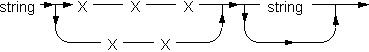
\includegraphics[width=0.6\linewidth]{figures/syntax-string.png}	
	\end{center}

\end{frame}

\begin{frame}[fragile]{Rekursion}

	Haskell:
	\begin{lstlisting}[gobble=4,language=Haskell]
		factorial 0 = 1
		factorial n = n * factorial (n - 1)
	\end{lstlisting}
	
	\vspace{2ex}
	
	C:
	\begin{lstlisting}[gobble=4]
		int factorial(int n) {
			if (n == 0) {
				return 1;
			}
			return n * factorial(n - 1);
		}
	\end{lstlisting}

\end{frame}

\begin{frame}[fragile]{Rekursion}
	
	\begin{itemize}
		\item Ende der Rekursion im trivialen Fall
		\item Im nicht-trivialen Fall \emp{Reduktion} in Richtung des trivialen Falls
	\end{itemize}

	\begin{minipage}{0.4\linewidth}
	\begin{lstlisting}[gobble=4]
		int factorial(int n) {
			if (n == 0) {
				return 1;
			}
			return n * factorial(n - 1);
		}
	\end{lstlisting}
	\end{minipage}%
	\begin{minipage}{0.6\linewidth}
	\begin{lstlisting}[gobble=6,showtabs=true,tab=$\mid$,tabsize=3]
		factorial(3) 
			return 3 * factorial(2)
			factorial(2) 
				return 2 * factorial(1) 
				factorial(1) 
					return 1 * factorial(0)
					factorial(0)
						return 1 
					return 1 * 1 = 1
				return 2 * 1 = 2 
			return 3 * 2 = 6 
	\end{lstlisting}
	\end{minipage}

\end{frame}


	% end of presentation
	%%%%%%%%%%%%%%%%%%%%%%%%%%%%%%%%%%%%%%%%%%%%%%%%%%%%%%%%%%%%%%%%%%%%%%%
	% backup slides
	
	\appendix
	\newcounter{finalframe}
	\setcounter{finalframe}{\value{framenumber}}
	
	%%%%%%%%%%%%%%%%%%%%%%%%%%%%%%%%%%%%%%%%%%%%%%%%%%%%%%%%%%%%%%%%%%%%%%%
	% end of backup slides
	\setcounter{framenumber}{\value{finalframe}}
\end{document}

